\documentclass[11pt,letterpaper]{article}
\usepackage[margin=1in]{geometry}
\usepackage{graphicx}
\usepackage{hyperref}
\usepackage{listings}
\usepackage{amsmath}
\pagestyle{headings}
\usepackage{epstopdf}

\begin{document}

\title{PHY 410 \\ Homework Assignment 9}
\author{Han Wen \\ \tiny Person No. 50096432}
\date{\today}

\maketitle

\begin{abstract}
The goal of this assignment is to get more familiar with PDE, as well as its application on typical mathematical physics equations


\end{abstract}

\tableofcontents

\newpage
\section{Problem 1}

\subsection{Description}

Compute the electrostatic potential due to an electric dipole in a two-dimensional grounded metal box and compare with the expected exact solution (sum of the Coulomb potentials of two point charges) in a box of infinite size. Use at least two different methods (Jacobi/Gauss-Seidel, SOR, FFT, Multigrid).

\subsection{Numerical Analysis}


Change the charge density to that of a dipole, with number of interior points in x or y 100, desired accuracy 0.000001, for Jacobi method, it takes 9072 steps, 32.39s to finish, while using 
SOR method, it only takes 241 steps, 1.01s. Here is the result Fig ~\ref{figure1}
 
\begin{figure}
\begin{center}
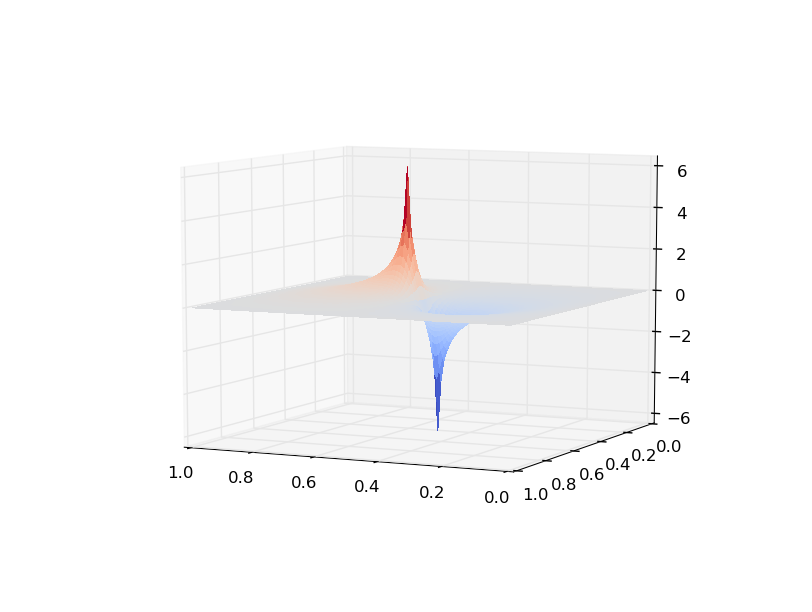
\includegraphics[width=0.8\linewidth,angle=0]{dipole1.png}
\caption{Electric potential for dipole}
\label{figure1}
\end{center}
\end{figure}









\newpage

\section{Problem 2}

\subsection{Description}
Use any wavepacket code to reproduce the movie frames in the article by Goldberg, Schey and Schwartz Am. J. Phys. 35, 177-186, 1967 or PDF copy. 
Modify the wavepacket code to study scattering from a potential of your choice. It might be most instructive to choose an example from your modern physics or quantum mechanics textbook. Describe the most interesting example you found.

\subsection{Result}

Firstly, I simulate the wavepacket when E=1.0 and 5.0. For E=1.0, the wavepacket frames: Fig. ~\ref{figure2}. For E=5.0, the frames: Fig. ~\ref{figure3}

\begin{figure}
\begin{center}
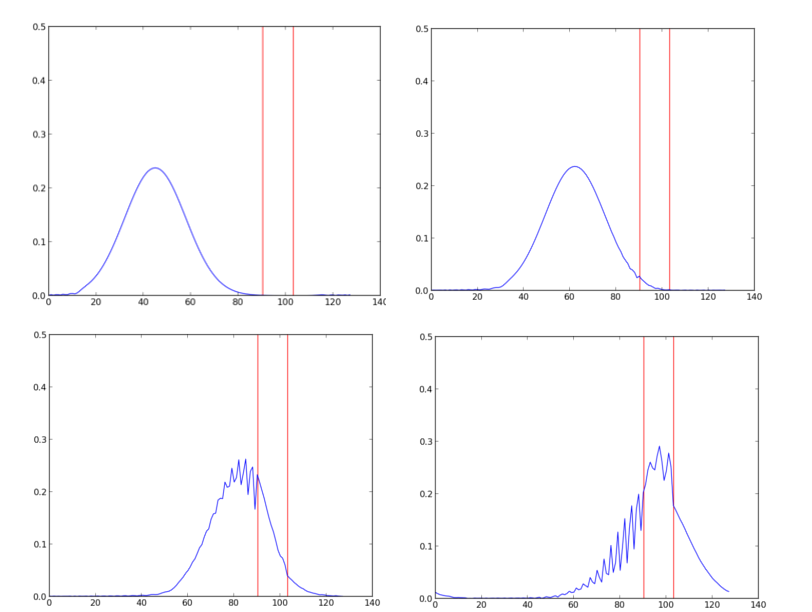
\includegraphics[width=0.8\linewidth,angle=0]{E1.png}
\caption{Wavepacket for E=1.0}
\label{figure2}
\end{center}
\end{figure}

\begin{figure}
\begin{center}
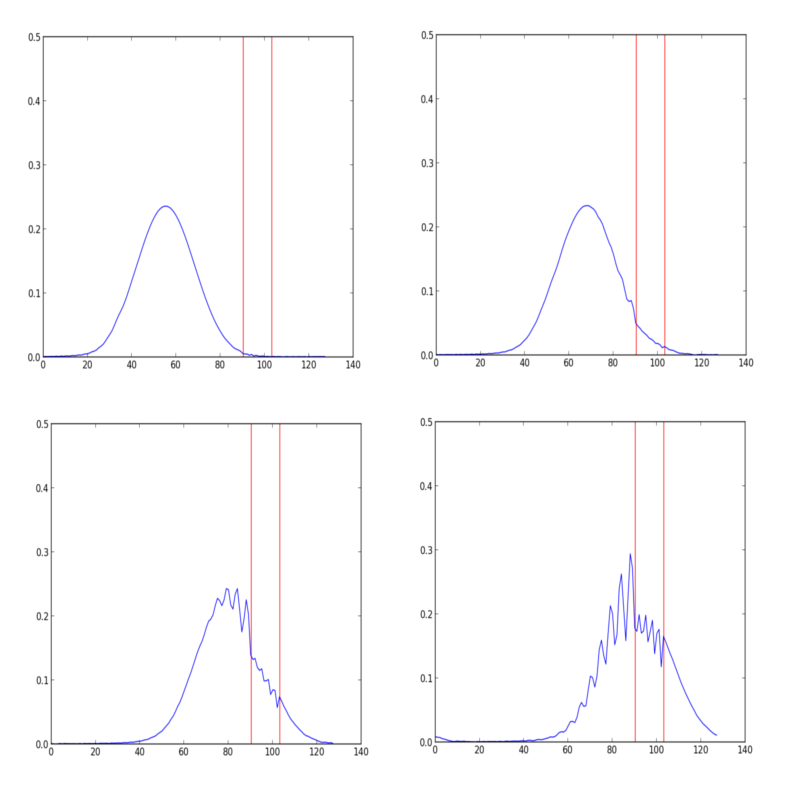
\includegraphics[width=0.8\linewidth,angle=0]{E5.png}
\caption{Wavepacket for E=5.0}
\label{figure3}
\end{center}
\end{figure}

Additionally, I chose the most common central potential, the column potential. And the result shows a wave run into the potential and then comes backwards, same as the real situation. Fig. ~\ref{figure4}

\begin{figure}
\begin{center}
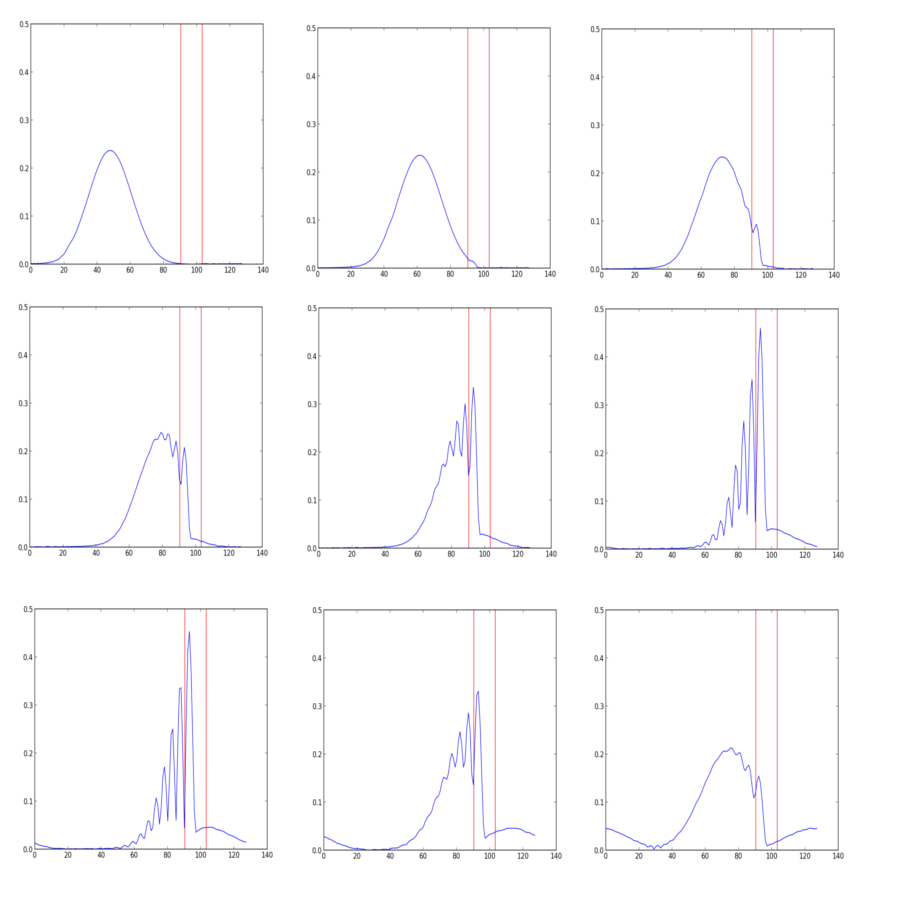
\includegraphics[width=0.8\linewidth,angle=0]{c.png}
\caption{Wavepacket for column potential}
\label{figure4}
\end{center}
\end{figure}

  
\section{Problem 3}
\subsection{Description}
In a wire chamber, several parallel wires are passed through a metal box. The wires are kept at a fixed potential V0, and the box edges are kept at ground. 

Assuming an infinitely long z-direction (so this reduces to a two-dimensional problem), extend Problem 1 to compute the electrostatic potential for 5 wires equally spaced through a box of x-direction length Lx = 10 and y-direction length Ly=2. 
Then, compute the trajectory of a charged particle traveling at a forty-five degree angle to the bottom of the box numerically. 

For the last part, you will have to pick one of the ODE methods (such as "kepler"), input the potential function that you have computed in this problem, and numerically take the gradient. This will be used as the derivative method. 


\subsection{Result}

By modifying the code, change the geometric parameters, I generated the potential shown here Fig. ~\ref{figure5}

Consequently, the trajectory of the particle is shown here Fig. ~\ref{figure6}. For simplicity, I set the v=1 in both x and y direction and took the gradient directly as the acceleration.

For v=5 in both direction, its behaviour is shown here: Fig. ~\ref{figure7}

\begin{figure}
\begin{center}
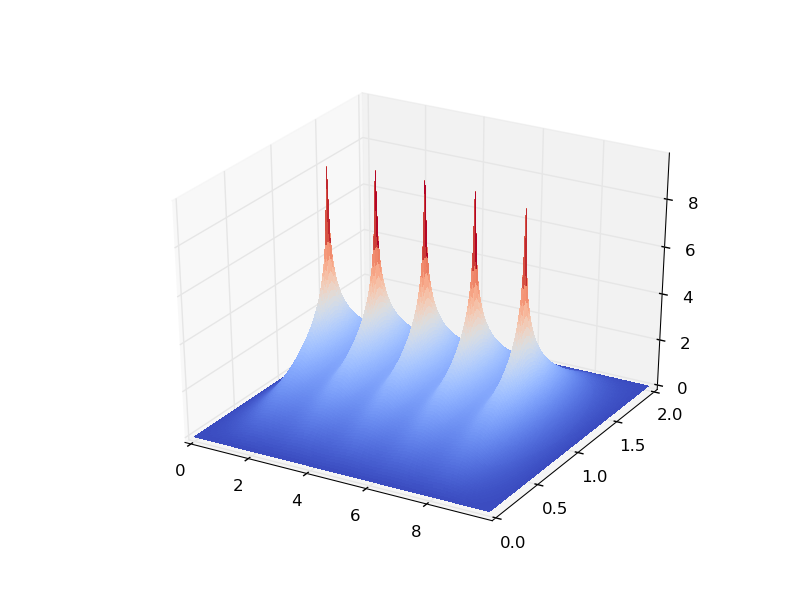
\includegraphics[width=0.8\linewidth,angle=0]{p3.png}
\caption{Potential of a wire chamber}
\label{figure5}
\end{center}
\end{figure}


\begin{figure}
\begin{center}
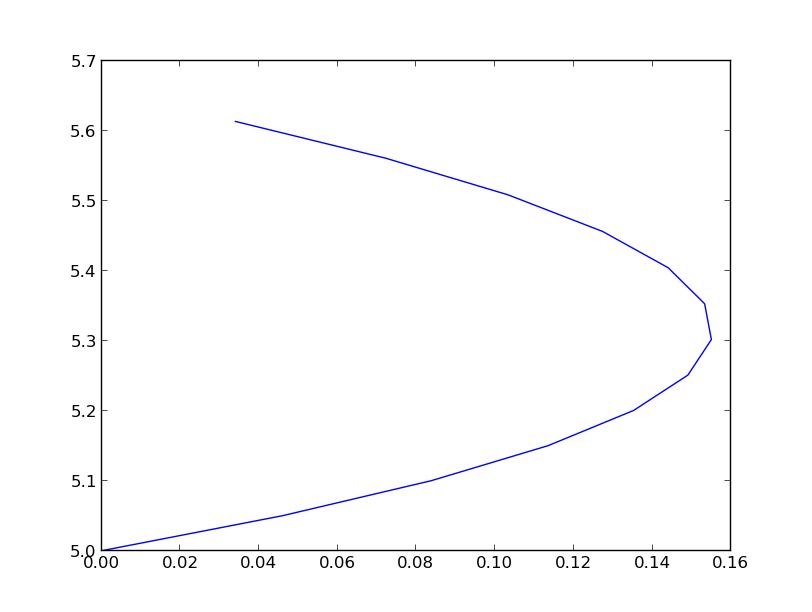
\includegraphics[width=0.8\linewidth,angle=0]{v11.png}
\caption{trajectory for v=1 in both direction}
\label{figure6}
\end{center}
\end{figure}

\begin{figure}
\begin{center}
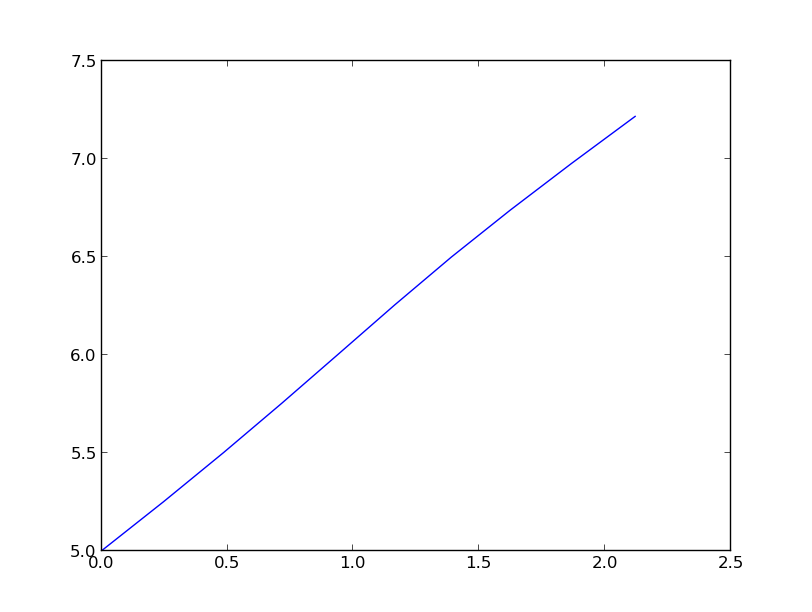
\includegraphics[width=0.8\linewidth,angle=0]{v55.png}
\caption{trajectory for v=5 in both direction}
\label{figure7}
\end{center}
\end{figure}


\newpage
\section*{Acknowledgements}

I discussed this assignment with my classmates and used material from the
cited references, but this write-up is my own.

\begin{thebibliography}{9}


\bibitem{coursepage}
PHY 410-505 Webpage, \url{http://www.physics.buffalo.edu/phy410-505}.



\end{thebibliography}

\newpage
\appendix
\section{Appendix}

\subsection{python code}

The following python code was used to obtain the results in this report:

\lstinputlisting[language=c++]{poisson1.cpp}

\lstinputlisting[language=python]{wavepacket.py}

\lstinputlisting[language=python]{poissontr.py}



\end{document}
